% Options for packages loaded elsewhere
\PassOptionsToPackage{unicode}{hyperref}
\PassOptionsToPackage{hyphens}{url}
\PassOptionsToPackage{dvipsnames,svgnames*,x11names*}{xcolor}
%
\documentclass[
  10pt,
]{article}
\usepackage{lmodern}
\usepackage{amsmath}
\usepackage{ifxetex,ifluatex}
\ifnum 0\ifxetex 1\fi\ifluatex 1\fi=0 % if pdftex
  \usepackage[T1]{fontenc}
  \usepackage[utf8]{inputenc}
  \usepackage{textcomp} % provide euro and other symbols
  \usepackage{amssymb}
\else % if luatex or xetex
  \usepackage{unicode-math}
  \defaultfontfeatures{Scale=MatchLowercase}
  \defaultfontfeatures[\rmfamily]{Ligatures=TeX,Scale=1}
\fi
% Use upquote if available, for straight quotes in verbatim environments
\IfFileExists{upquote.sty}{\usepackage{upquote}}{}
\IfFileExists{microtype.sty}{% use microtype if available
  \usepackage[]{microtype}
  \UseMicrotypeSet[protrusion]{basicmath} % disable protrusion for tt fonts
}{}
\makeatletter
\@ifundefined{KOMAClassName}{% if non-KOMA class
  \IfFileExists{parskip.sty}{%
    \usepackage{parskip}
  }{% else
    \setlength{\parindent}{0pt}
    \setlength{\parskip}{6pt plus 2pt minus 1pt}}
}{% if KOMA class
  \KOMAoptions{parskip=half}}
\makeatother
\usepackage{xcolor}
\IfFileExists{xurl.sty}{\usepackage{xurl}}{} % add URL line breaks if available
\IfFileExists{bookmark.sty}{\usepackage{bookmark}}{\usepackage{hyperref}}
\hypersetup{
  pdftitle={Using R tools for analysis  of primary biodiversity data provided by SBDI},
  pdfauthor={Debora Arlt and Alejandro Ruete  for the Swedish Biodiversity Data Infrastructure},
  colorlinks=true,
  linkcolor=Maroon,
  filecolor=Maroon,
  citecolor=Blue,
  urlcolor=Blue,
  pdfcreator={LaTeX via pandoc}}
\urlstyle{same} % disable monospaced font for URLs
\usepackage[margin=1in]{geometry}
\usepackage{color}
\usepackage{fancyvrb}
\newcommand{\VerbBar}{|}
\newcommand{\VERB}{\Verb[commandchars=\\\{\}]}
\DefineVerbatimEnvironment{Highlighting}{Verbatim}{commandchars=\\\{\}}
% Add ',fontsize=\small' for more characters per line
\usepackage{framed}
\definecolor{shadecolor}{RGB}{248,248,248}
\newenvironment{Shaded}{\begin{snugshade}}{\end{snugshade}}
\newcommand{\AlertTok}[1]{\textcolor[rgb]{0.94,0.16,0.16}{#1}}
\newcommand{\AnnotationTok}[1]{\textcolor[rgb]{0.56,0.35,0.01}{\textbf{\textit{#1}}}}
\newcommand{\AttributeTok}[1]{\textcolor[rgb]{0.77,0.63,0.00}{#1}}
\newcommand{\BaseNTok}[1]{\textcolor[rgb]{0.00,0.00,0.81}{#1}}
\newcommand{\BuiltInTok}[1]{#1}
\newcommand{\CharTok}[1]{\textcolor[rgb]{0.31,0.60,0.02}{#1}}
\newcommand{\CommentTok}[1]{\textcolor[rgb]{0.56,0.35,0.01}{\textit{#1}}}
\newcommand{\CommentVarTok}[1]{\textcolor[rgb]{0.56,0.35,0.01}{\textbf{\textit{#1}}}}
\newcommand{\ConstantTok}[1]{\textcolor[rgb]{0.00,0.00,0.00}{#1}}
\newcommand{\ControlFlowTok}[1]{\textcolor[rgb]{0.13,0.29,0.53}{\textbf{#1}}}
\newcommand{\DataTypeTok}[1]{\textcolor[rgb]{0.13,0.29,0.53}{#1}}
\newcommand{\DecValTok}[1]{\textcolor[rgb]{0.00,0.00,0.81}{#1}}
\newcommand{\DocumentationTok}[1]{\textcolor[rgb]{0.56,0.35,0.01}{\textbf{\textit{#1}}}}
\newcommand{\ErrorTok}[1]{\textcolor[rgb]{0.64,0.00,0.00}{\textbf{#1}}}
\newcommand{\ExtensionTok}[1]{#1}
\newcommand{\FloatTok}[1]{\textcolor[rgb]{0.00,0.00,0.81}{#1}}
\newcommand{\FunctionTok}[1]{\textcolor[rgb]{0.00,0.00,0.00}{#1}}
\newcommand{\ImportTok}[1]{#1}
\newcommand{\InformationTok}[1]{\textcolor[rgb]{0.56,0.35,0.01}{\textbf{\textit{#1}}}}
\newcommand{\KeywordTok}[1]{\textcolor[rgb]{0.13,0.29,0.53}{\textbf{#1}}}
\newcommand{\NormalTok}[1]{#1}
\newcommand{\OperatorTok}[1]{\textcolor[rgb]{0.81,0.36,0.00}{\textbf{#1}}}
\newcommand{\OtherTok}[1]{\textcolor[rgb]{0.56,0.35,0.01}{#1}}
\newcommand{\PreprocessorTok}[1]{\textcolor[rgb]{0.56,0.35,0.01}{\textit{#1}}}
\newcommand{\RegionMarkerTok}[1]{#1}
\newcommand{\SpecialCharTok}[1]{\textcolor[rgb]{0.00,0.00,0.00}{#1}}
\newcommand{\SpecialStringTok}[1]{\textcolor[rgb]{0.31,0.60,0.02}{#1}}
\newcommand{\StringTok}[1]{\textcolor[rgb]{0.31,0.60,0.02}{#1}}
\newcommand{\VariableTok}[1]{\textcolor[rgb]{0.00,0.00,0.00}{#1}}
\newcommand{\VerbatimStringTok}[1]{\textcolor[rgb]{0.31,0.60,0.02}{#1}}
\newcommand{\WarningTok}[1]{\textcolor[rgb]{0.56,0.35,0.01}{\textbf{\textit{#1}}}}
\usepackage{longtable,booktabs}
\usepackage{calc} % for calculating minipage widths
% Correct order of tables after \paragraph or \subparagraph
\usepackage{etoolbox}
\makeatletter
\patchcmd\longtable{\par}{\if@noskipsec\mbox{}\fi\par}{}{}
\makeatother
% Allow footnotes in longtable head/foot
\IfFileExists{footnotehyper.sty}{\usepackage{footnotehyper}}{\usepackage{footnote}}
\makesavenoteenv{longtable}
\usepackage{graphicx}
\makeatletter
\def\maxwidth{\ifdim\Gin@nat@width>\linewidth\linewidth\else\Gin@nat@width\fi}
\def\maxheight{\ifdim\Gin@nat@height>\textheight\textheight\else\Gin@nat@height\fi}
\makeatother
% Scale images if necessary, so that they will not overflow the page
% margins by default, and it is still possible to overwrite the defaults
% using explicit options in \includegraphics[width, height, ...]{}
\setkeys{Gin}{width=\maxwidth,height=\maxheight,keepaspectratio}
% Set default figure placement to htbp
\makeatletter
\def\fps@figure{htbp}
\makeatother
\setlength{\emergencystretch}{3em} % prevent overfull lines
\providecommand{\tightlist}{%
  \setlength{\itemsep}{0pt}\setlength{\parskip}{0pt}}
\setcounter{secnumdepth}{5}
\ifluatex
  \usepackage{selnolig}  % disable illegal ligatures
\fi
\usepackage[]{natbib}
\bibliographystyle{apalike}

\title{Using R tools for analysis of primary biodiversity data provided by SBDI}
\author{Debora Arlt and Alejandro Ruete for the Swedish Biodiversity Data Infrastructure}
\date{2021-05-26}

\begin{document}
\maketitle

{
\hypersetup{linkcolor=}
\setcounter{tocdepth}{2}
\tableofcontents
}
\hypertarget{introduction}{%
\section*{Introduction}\label{introduction}}
\addcontentsline{toc}{section}{Introduction}

Biodiversity resources are increasingly international. The SBDI has made an effort to canalize biodiversity data and resources to help the research community access and analyze Swedish primary biodiversity data. Each research question draws its own challenges which are unique in themselves. Our aim here is to provide a few examples that prompt questions that may be asked at different stages of the process. The validity and appropriateness of a particular method depends on the individual researcher(s). For a comprehensive workflow on how to treat and analyze PBD please refer to our tutorial on \href{https://github.com/biodiversitydata-se/biodiversity-analysis-tools}{biodiversity analysis tool} where we go through the complete workflow Data --\textgreater{} Cleaning --\textgreater{} Fitness evaluation --\textgreater{} Analysis

\hypertarget{r-and-mirroreum}{%
\subsection*{R and Mirroreum}\label{r-and-mirroreum}}
\addcontentsline{toc}{subsection}{R and Mirroreum}

The present tutorial is focused on the statistical programming language R.
R is a free software environment for statistical computing and graphics that is
widely used within the scientific community and where the complete analysis
workflow can be documented in a fully reproducible way.

At SBDI we provide access for researchers and students to \href{https://mirroreum.biodiversitydata.se/}{Mirroreum}
-- an online web-based environment for Reproducible Open Research in the area of
biodiversity analysis. Mirroreum is based on a Free and Open Source stack of software.
Logging in, you immediately get access to a web-based version of R Studio with a
large number of pre-installed packages such as all the packages offered from ROpenSci and more.

Compared to running R Studio on your own machine, Mirroreum offers more
computational resources and a standardized environment where you can rely on all
the relevant packages being installed and the configuration parameters being set
appropriately.
To know more about Mirroreum or to request an account please visit the \href{https://docs.biodiversitydata.se/analyse-data/mirroreum/}{SBDI documentation site}

\hypertarget{sbdi4r---r-package-to-search-an-access-data}{%
\subsection*{SBDI4R - R package to search an access data}\label{sbdi4r---r-package-to-search-an-access-data}}
\addcontentsline{toc}{subsection}{SBDI4R - R package to search an access data}

The SBDI4R package enables the R community to directly access data and resources
hosted by SBDI. The goal is to enable observations of species to be
queried and output in a range of standard formats. It includes some filter functions
that allow you to filter prior to download. It also includes some simple summary
functions, and some function for some simple data exploration. The examples
included in this tutorial also show you how you can continue exploring and analyzing
using other R package.

Please refer to the \href{https://biodiversitydata-se.github.io/SBDI4R}{package documentation}
for details on how to install it. Once installed the SBDI4R package must be loaded
for each new R session:

\begin{Shaded}
\begin{Highlighting}[]
\FunctionTok{library}\NormalTok{(SBDI4R)}
\end{Highlighting}
\end{Shaded}

\hypertarget{customizing-sbdi4r}{%
\subsection*{Customizing SBDI4R}\label{customizing-sbdi4r}}
\addcontentsline{toc}{subsection}{Customizing SBDI4R}

Various aspects of the SBDI4R package can be customized.

\hypertarget{caching}{%
\subsubsection*{Caching}\label{caching}}
\addcontentsline{toc}{subsubsection}{Caching}

SBDI4R can cache most results to local files. This means that if the
same code is run multiple times, the second and subsequent iterations
will be faster. This will also reduce load on the web servers. By
default, this caching is session-based, meaning that the local files are
stored in a temporary directory that is automatically deleted when the R
session is ended. This behaviour can be altered so that caching is
permanent, by setting the caching directory to a non-temporary location.
For example, under Windows, use something like:

\begin{Shaded}
\begin{Highlighting}[]
\FunctionTok{sbdi\_config}\NormalTok{(}\AttributeTok{cache\_directory =} \FunctionTok{file.path}\NormalTok{(}\StringTok{"c:"}\NormalTok{,}\StringTok{"mydata"}\NormalTok{,}\StringTok{"sbdi\_cache"}\NormalTok{)) }\DocumentationTok{\#\# Windows}
\end{Highlighting}
\end{Shaded}

or for Linux:

\begin{Shaded}
\begin{Highlighting}[]
\FunctionTok{sbdi\_config}\NormalTok{(}\AttributeTok{cache\_directory =} \StringTok{"\textasciitilde{}/mydata/sbdi\_cache"}\NormalTok{) }\DocumentationTok{\#\# Linux}
\end{Highlighting}
\end{Shaded}

Note that this directory must exist (you need to create it yourself).

All results will be stored in that cache directory and will be used from
one session to the next. They won't be re-downloaded from the server
unless the user specifically deletes those files or changes the caching
setting to ``refresh''.

If you change the cache\_directory to a permanent location, you may wish
to add something like this to your .Rprofile file, so that it happens
automatically each time the SBDI4R package is loaded:

\begin{Shaded}
\begin{Highlighting}[]
\FunctionTok{setHook}\NormalTok{(}\FunctionTok{packageEvent}\NormalTok{(}\StringTok{"SBDI4R"}\NormalTok{, }\StringTok{"onLoad"}\NormalTok{), }
        \ControlFlowTok{function}\NormalTok{(...) }\FunctionTok{sbdi\_config}\NormalTok{(}\AttributeTok{cache\_directory=}\FunctionTok{file.path}\NormalTok{(}\StringTok{"\textasciitilde{}"}\NormalTok{,}\StringTok{"mydata"}\NormalTok{,}\StringTok{"sbdi\_cache"}\NormalTok{)))}
\end{Highlighting}
\end{Shaded}

Caching can also be turned off entirely by:

\begin{Shaded}
\begin{Highlighting}[]
\FunctionTok{sbdi\_config}\NormalTok{(}\AttributeTok{caching=}\StringTok{"off"}\NormalTok{)}
\end{Highlighting}
\end{Shaded}

or set to ``refresh'', meaning that the cached results will re-downloaded
from the SBDI servers and the cache updated. (This will happen for as
long as caching is set to ``refresh'' --- so you may wish to switch back to
normal ``on'' caching behavior once you have updated your cache with the
data you are working on).

\hypertarget{e-mail-address}{%
\subsubsection*{E-mail address}\label{e-mail-address}}
\addcontentsline{toc}{subsubsection}{E-mail address}

Each download request to SBDI servers is also accompanied by an ``e-mail address''
string that identifies the user making the request. You will need to provide an
email address registered with the SBDI. You can create an account
\href{https://auth.biodiversitydata.se/cas/login}{here}. Once an email is registered
with the SBDI, it should be stored in the config:

\begin{Shaded}
\begin{Highlighting}[]
\FunctionTok{sbdi\_config}\NormalTok{(}\AttributeTok{email=}\StringTok{"your.valid@emailaddress.com"}\NormalTok{)}
\end{Highlighting}
\end{Shaded}

Else you can provide this e-mail address as a parameter directly to
each call of the function occurrences().

\hypertarget{setting-the-download-reason}{%
\subsubsection*{Setting the download reason}\label{setting-the-download-reason}}
\addcontentsline{toc}{subsubsection}{Setting the download reason}

SBDI requires that you provide a reason when downloading occurrence data
(via the SBDI4R \texttt{occurrences()} function). You can provide this as a
parameter directly to each call of \texttt{occurrences()}, or you can set it
once per session using:

\begin{Shaded}
\begin{Highlighting}[]
\FunctionTok{sbdi\_config}\NormalTok{(}\AttributeTok{download\_reason\_id =} \StringTok{"your\_reason\_id"}\NormalTok{)}
\end{Highlighting}
\end{Shaded}

(See \texttt{sbdi\_reasons()} for valid download reasons, e.g.
* 3 for ``education'',
* 7 for ``ecological research'',
* 8 for ``systematic research/taxonomy'',
* 10 for ``testing'')

\emph{NO} other personal identification information is sent. You can see all
configuration settings, including the the user-agent string that is
being used, with the command:

\begin{Shaded}
\begin{Highlighting}[]
\FunctionTok{sbdi\_config}\NormalTok{()}
\end{Highlighting}
\end{Shaded}

\hypertarget{other-options}{%
\subsubsection*{Other options}\label{other-options}}
\addcontentsline{toc}{subsubsection}{Other options}

If you make a request that returns an empty result set (e.g.~an
un-matched name), by default you will simply get an empty data structure
returned to you without any special notification. If you would like to
be warned about empty result sets, you can use:

\begin{Shaded}
\begin{Highlighting}[]
\FunctionTok{sbdi\_config}\NormalTok{(}\AttributeTok{warn\_on\_empty=}\ConstantTok{TRUE}\NormalTok{)}
\end{Highlighting}
\end{Shaded}

\hypertarget{other-packages-needed}{%
\subsection*{Other packages needed}\label{other-packages-needed}}
\addcontentsline{toc}{subsection}{Other packages needed}

Some additional packages are needed for these examples. Install them if necessary
with the following script.

\begin{Shaded}
\begin{Highlighting}[]
\NormalTok{to\_install }\OtherTok{\textless{}{-}} \FunctionTok{c}\NormalTok{(}\StringTok{"dplyr"}\NormalTok{, }\StringTok{"BIRDS"}\NormalTok{,}\StringTok{"ggplot2"}\NormalTok{, }\StringTok{"jpeg"}\NormalTok{, }\StringTok{"leaflet"}\NormalTok{,}\StringTok{"maps"}\NormalTok{, }\StringTok{"mapdata"}\NormalTok{,}
                \StringTok{"maptools"}\NormalTok{, }\StringTok{"sp"}\NormalTok{, }\StringTok{"rgeos"}\NormalTok{, }\StringTok{"tidyr"}\NormalTok{, }\StringTok{"vegan"}\NormalTok{)}
\NormalTok{to\_install }\OtherTok{\textless{}{-}}\NormalTok{ to\_install[}\SpecialCharTok{!}\FunctionTok{sapply}\NormalTok{(to\_install, requireNamespace, }\AttributeTok{quietly=}\ConstantTok{TRUE}\NormalTok{)]}
\ControlFlowTok{if}\NormalTok{(}\FunctionTok{length}\NormalTok{(to\_install)}\SpecialCharTok{\textgreater{}}\DecValTok{0}\NormalTok{)}
    \FunctionTok{install.packages}\NormalTok{(to\_install, }\AttributeTok{repos=}\StringTok{"http://cran.us.r{-}project.org"}\NormalTok{)}
\end{Highlighting}
\end{Shaded}

\hypertarget{your-collaboration-is-appreciated}{%
\subsection*{Your collaboration is appreciated}\label{your-collaboration-is-appreciated}}
\addcontentsline{toc}{subsection}{Your collaboration is appreciated}

Open Source also means that you can contribute. You don't need to know how to program
but every input is appreciated. Did you find something that is not working?
Have suggestions for examples or text? you can always
1. Reach to us via the \href{https://docs.biodiversitydata.se/support/}{support center}
2. Submit and issue to the GitHub code repository \href{https://docs.github.com/en/github/managing-your-work-on-github/managing-your-work-with-issues-and-pull-requests/creating-an-issue}{see how}
3. Or contribute with your code or documents modifications by \href{https://docs.github.com/en/github/getting-started-with-github/quickstart/fork-a-repo}{``forking''}
the code and submitting a \href{https://docs.github.com/en/github/collaborating-with-issues-and-pull-requests/proposing-changes-to-your-work-with-pull-requests/creating-a-pull-request-from-a-fork}{``pull request''}

The repositories you can contribute to are:
* Mirroreum \url{https://github.com/mskyttner/mirroreum}
* SBDI4R \url{https://github.com/biodiversitydata-se/SBDI4R} (NOTE: we may not develop this package but instead move to a new one)
* the general analysis workflows {[}\url{https://github.com/biodiversitydata-se/biodiversity-analysis-tools}{]} \url{https://github.com/biodiversitydata-se/biodiversity-analysis-tools}
* these tutorial \url{https://github.com/biodiversitydata-se/r-tools-tutorial}

\hypertarget{example-with-fish-data-from-sers}{%
\section{Example with fish data from SERS}\label{example-with-fish-data-from-sers}}

In this example we are interested in exploring data from a specific data resource -- Swedish Electrofishing Registry - SERS (Institutionen för akvatiska resurser, SLU). This data base has 2.8 M observations starting in the 1950's.

As you may already know, SBDI is a collection of many biodiversity databases. We start by searching for the data resource we are interested in using the function \texttt{pick\_filter()}. This is an interactive query guiding you through the many resources available to filtering your query (data resources, spatial layers, and curated species lists).

\begin{Shaded}
\begin{Highlighting}[]
\FunctionTok{library}\NormalTok{(SBDI4R)}
\NormalTok{fq\_str }\OtherTok{\textless{}{-}} \FunctionTok{pick\_filter}\NormalTok{(}\StringTok{"resource"}\NormalTok{) }
\CommentTok{\# follow the instructions }
\end{Highlighting}
\end{Shaded}

Follow the instruction. Your choices here would have been ``in3'' --\textgreater{} ``dr10''. Your variable \texttt{fq\_str} will now contain a string ``data\_resource\_uid:dr10''.

But we are not interested in the complete database, but on the last 10 years of data. for this we concatenate (add to a vector) another filter string. These will be treated as AND factors.

\begin{Shaded}
\begin{Highlighting}[]
\NormalTok{y1 }\OtherTok{\textless{}{-}} \DecValTok{2008}
\NormalTok{y2 }\OtherTok{\textless{}{-}} \DecValTok{2012}
\NormalTok{fq\_str }\OtherTok{\textless{}{-}} \FunctionTok{c}\NormalTok{(fq\_str, }\FunctionTok{paste0}\NormalTok{(}\StringTok{"year:["}\NormalTok{, y1, }\StringTok{" TO "}\NormalTok{, y2,}\StringTok{"]"}\NormalTok{))}
\CommentTok{\# Note the square brackets are hard limits}
\end{Highlighting}
\end{Shaded}

For references on how to use the filters see SBDI APIS \href{https://api.biodiversitydata.se/?lang=en-US\#ws3}{documentation}.

Using the function \texttt{occurrences()} we can the query for the observations fulfilling our filter. If you haven't specified that in the \texttt{sbdi\_config()} before, you need to pass your email and the download reason.

\begin{Shaded}
\begin{Highlighting}[]
\FunctionTok{library}\NormalTok{(SBDI4R)}
\NormalTok{xf }\OtherTok{\textless{}{-}} \FunctionTok{occurrences}\NormalTok{(}\AttributeTok{fq =}\NormalTok{ fq\_str,}
                 \AttributeTok{email =} \StringTok{"sbdi4r{-}test@biodiversitydata.se"}\NormalTok{, }
                 \AttributeTok{download\_reason\_id =} \DecValTok{10}\NormalTok{)}
\end{Highlighting}
\end{Shaded}

\begin{verbatim}
## Registered S3 methods overwritten by 'ALA4R':
##   method              from  
##   subset.occurrences  SBDI4R
##   summary.occurrences SBDI4R
##   unique.occurrences  SBDI4R
\end{verbatim}

\begin{Shaded}
\begin{Highlighting}[]
\CommentTok{\# Simply summarise all records by data source }
\FunctionTok{table}\NormalTok{(xf}\SpecialCharTok{$}\NormalTok{data}\SpecialCharTok{$}\NormalTok{dataResourceName)}
\end{Highlighting}
\end{Shaded}

\begin{verbatim}
## 
## SLU Aqua  Institute of Freshwater Research Swedish Electrofishing Registry - SERS 
##                                                                             95082
\end{verbatim}

\begin{Shaded}
\begin{Highlighting}[]
\FunctionTok{table}\NormalTok{(xf}\SpecialCharTok{$}\NormalTok{data}\SpecialCharTok{$}\NormalTok{dataResourceID)}
\end{Highlighting}
\end{Shaded}

\begin{verbatim}
## 
##  dr10 
## 95082
\end{verbatim}

\hypertarget{plotting-data-on-a-map}{%
\subsection{Plotting data on a map}\label{plotting-data-on-a-map}}

You can quickly plot all the observations as a PDF file with the function \texttt{ocurrence\_plot()}, one page per species:

\begin{Shaded}
\begin{Highlighting}[]
\FunctionTok{occurrences\_plot}\NormalTok{(xf, }\StringTok{"obsPlot.pdf"}\NormalTok{, }
                 \AttributeTok{grouped=}\ConstantTok{FALSE}\NormalTok{, }
                 \AttributeTok{taxon\_level=}\StringTok{"species"}\NormalTok{, }
                 \AttributeTok{pch=}\StringTok{\textquotesingle{}+\textquotesingle{}}\NormalTok{)}
\end{Highlighting}
\end{Shaded}

Note that the plot is saved to a pdf file in the current working directory. You can find that with \texttt{getwd()}.

\hypertarget{leaflet}{%
\paragraph{Leaflet}\label{leaflet}}

There are many other ways of producing spatial plots in R. The leaflet package provides a simple method of producing browser-based maps with panning, zooming, and background layers:

\begin{Shaded}
\begin{Highlighting}[]
\FunctionTok{library}\NormalTok{(leaflet)}
\CommentTok{\# drop any records with missing lat/lon values}
\NormalTok{xfl }\OtherTok{\textless{}{-}}\NormalTok{ xf}\SpecialCharTok{$}\NormalTok{data[}\SpecialCharTok{!}\FunctionTok{is.na}\NormalTok{(xf}\SpecialCharTok{$}\NormalTok{data}\SpecialCharTok{$}\NormalTok{longitude) }\SpecialCharTok{|} \SpecialCharTok{!}\FunctionTok{is.na}\NormalTok{(xf}\SpecialCharTok{$}\NormalTok{data}\SpecialCharTok{$}\NormalTok{latitude),] }
\NormalTok{marker\_colour }\OtherTok{\textless{}{-}} \FunctionTok{rep}\NormalTok{(}\StringTok{"\#d95f02"}\NormalTok{, }\FunctionTok{nrow}\NormalTok{(xfl))}
\CommentTok{\# blank map, with imagery background}
\FunctionTok{leaflet}\NormalTok{(}\AttributeTok{width =} \StringTok{"100\%"}\NormalTok{) }\SpecialCharTok{\%\textgreater{}\%} 
  \FunctionTok{addProviderTiles}\NormalTok{(}\StringTok{"Esri.WorldImagery"}\NormalTok{) }\SpecialCharTok{\%\textgreater{}\%}
  \CommentTok{\# add markers}
  \FunctionTok{addCircleMarkers}\NormalTok{(xfl}\SpecialCharTok{$}\NormalTok{longitude, xfl}\SpecialCharTok{$}\NormalTok{latitude,  }
                   \AttributeTok{radius =} \DecValTok{1}\NormalTok{, }
                   \AttributeTok{fillOpacity =}\NormalTok{.}\DecValTok{5}\NormalTok{, }
                   \AttributeTok{opacity =} \DecValTok{1}\NormalTok{,}
                   \AttributeTok{col=}\NormalTok{marker\_colour,}
                  \AttributeTok{clusterOptions =} \FunctionTok{markerClusterOptions}\NormalTok{())}
\end{Highlighting}
\end{Shaded}

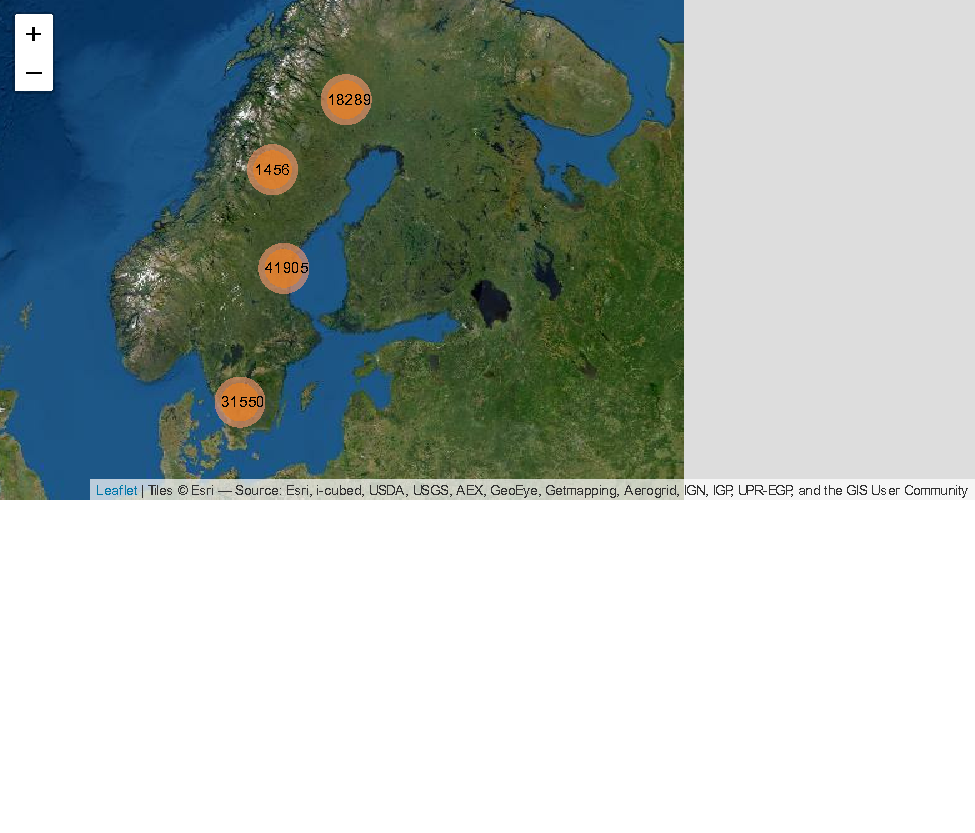
\includegraphics{r-tools-tutorial_files/figure-latex/leaflet-1.pdf}

\hypertarget{temporal-summary}{%
\subsection{Temporal summary}\label{temporal-summary}}

A quick summary over the years reveal a drop in number of records over time.

\begin{Shaded}
\begin{Highlighting}[]
\FunctionTok{table}\NormalTok{(xf}\SpecialCharTok{$}\NormalTok{data}\SpecialCharTok{$}\NormalTok{year)}
\end{Highlighting}
\end{Shaded}

\begin{verbatim}
## 
##  2008  2009  2010  2011  2012 
## 18168 19674 20055 17188 19997
\end{verbatim}

\begin{Shaded}
\begin{Highlighting}[]
\FunctionTok{hist}\NormalTok{(xf}\SpecialCharTok{$}\NormalTok{data}\SpecialCharTok{$}\NormalTok{year, }
     \AttributeTok{breaks =} \FunctionTok{seq}\NormalTok{(y1, y2), }
     \AttributeTok{xlab =} \StringTok{"Year"}\NormalTok{, }
     \AttributeTok{main =} \StringTok{""}\NormalTok{)}
\end{Highlighting}
\end{Shaded}

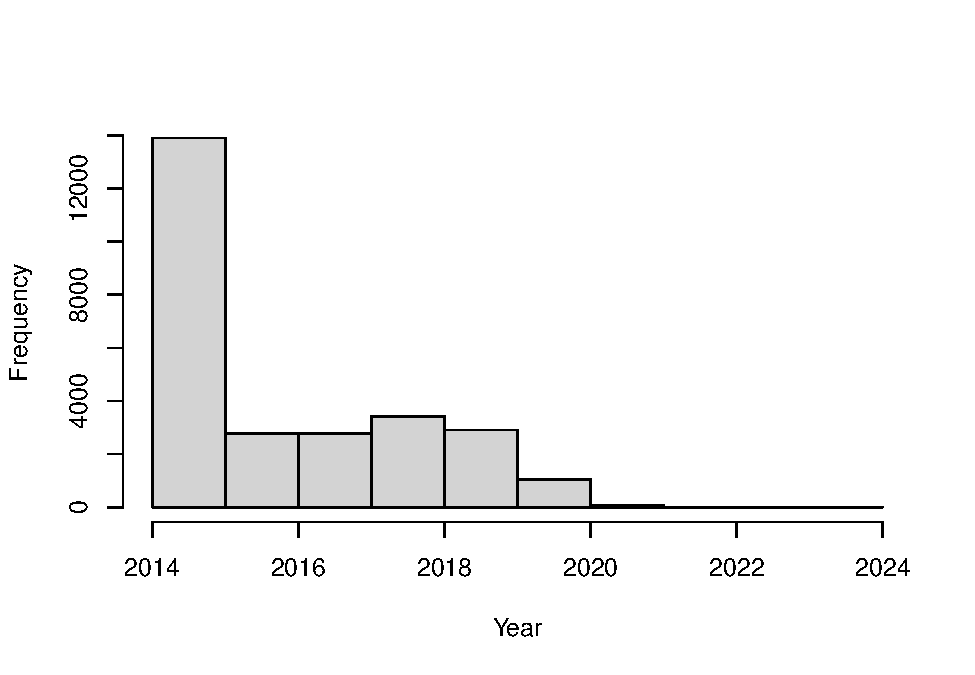
\includegraphics{r-tools-tutorial_files/figure-latex/timeHist-1.pdf}

\hypertarget{species-summary}{%
\subsection{Species summary}\label{species-summary}}

In the same way we can summaries the number of observations for each species, by common or scientific name.

\begin{Shaded}
\begin{Highlighting}[]
\NormalTok{sppTab }\OtherTok{\textless{}{-}} \FunctionTok{table}\NormalTok{(xf}\SpecialCharTok{$}\NormalTok{data}\SpecialCharTok{$}\NormalTok{commonName)}
\NormalTok{sppDF }\OtherTok{\textless{}{-}} \FunctionTok{as.data.frame}\NormalTok{(sppTab)}
\FunctionTok{colnames}\NormalTok{(sppDF)[}\DecValTok{1}\NormalTok{] }\OtherTok{\textless{}{-}} \StringTok{"species"}
\FunctionTok{head}\NormalTok{(sppDF)}
\end{Highlighting}
\end{Shaded}

\begin{verbatim}
##           species Freq
## 1                   66
## 2 Alpine bullhead 4615
## 3 American burbot 7081
## 4        Aral asp    6
## 5     Arctic char   46
## 6    aurora trout  856
\end{verbatim}

\begin{Shaded}
\begin{Highlighting}[]
\NormalTok{sppTab }\OtherTok{\textless{}{-}} \FunctionTok{table}\NormalTok{(xf}\SpecialCharTok{$}\NormalTok{data}\SpecialCharTok{$}\NormalTok{scientificName)}
\NormalTok{sppDF }\OtherTok{\textless{}{-}} \FunctionTok{as.data.frame}\NormalTok{(sppTab)}
\FunctionTok{colnames}\NormalTok{(sppDF)[}\DecValTok{1}\NormalTok{] }\OtherTok{\textless{}{-}} \StringTok{"species"}
\FunctionTok{head}\NormalTok{(sppDF)}
\end{Highlighting}
\end{Shaded}

\begin{verbatim}
##                                species Freq
## 1       Abramis brama (Linnaeus, 1758)   61
## 2   Alburnus alburnus (Linnaeus, 1758)  660
## 3   Anguilla anguilla (Linnaeus, 1758) 2140
## 4                            Astacidae  100
## 5     Astacus astacus (Linnaeus, 1758)  618
## 6 Barbatula barbatula (Linnaeus, 1758)  620
\end{verbatim}

Perhaps, you need to send this table as a .CSV file to a colleague.

\begin{Shaded}
\begin{Highlighting}[]
\FunctionTok{write.csv}\NormalTok{(sppDF, }\StringTok{"SERS\_species\_summary.csv"}\NormalTok{)}
\CommentTok{\# }\AlertTok{NOTE}\CommentTok{: again this will be saved on your working directory}
\end{Highlighting}
\end{Shaded}

\hypertarget{spatial-biodiversity-analysis}{%
\subsection{Spatial biodiversity analysis}\label{spatial-biodiversity-analysis}}

Let's now ask: how does the species richness vary across Sweden? In this case we want to summarise occurrences species-wise over a defined grid instead of plotting every observation point. First we need to overlay the observations with a grid. In this case, the standard Swedish grids at 50, 25, 10 and 5 km are provided as data in the SBDI4R package (with Coordinate Reference System = WGS84, EPSG:4326).

\begin{Shaded}
\begin{Highlighting}[]
\FunctionTok{library}\NormalTok{(sp) }\CommentTok{\# the function coordinates() and proj4string() are in sp}
\end{Highlighting}
\end{Shaded}

\begin{verbatim}
## Warning: package 'sp' was built under R version 4.0.3
\end{verbatim}

\begin{Shaded}
\begin{Highlighting}[]
\FunctionTok{library}\NormalTok{(rgeos) }\CommentTok{\# the function over() is in package rgeos}
\end{Highlighting}
\end{Shaded}

\begin{verbatim}
## rgeos version: 0.5-5, (SVN revision 640)
##  GEOS runtime version: 3.8.0-CAPI-1.13.1 
##  Linking to sp version: 1.4-2 
##  Polygon checking: TRUE
\end{verbatim}

\begin{Shaded}
\begin{Highlighting}[]
\CommentTok{\# load some shapes over Sweden\textquotesingle{}s political borders}
\FunctionTok{data}\NormalTok{(}\StringTok{"swe\_wgs84"}\NormalTok{, }\AttributeTok{package=}\StringTok{"SBDI4R"}\NormalTok{, }\AttributeTok{envir=}\FunctionTok{environment}\NormalTok{())}
\CommentTok{\# A standard 50km grid}
\FunctionTok{data}\NormalTok{(}\StringTok{"Sweden\_Grid\_50km\_Wgs84"}\NormalTok{, }\AttributeTok{package=}\StringTok{"SBDI4R"}\NormalTok{, }\AttributeTok{envir=}\FunctionTok{environment}\NormalTok{())}

\NormalTok{grid }\OtherTok{\textless{}{-}}\NormalTok{ Sweden\_Grid\_50km\_Wgs84}

\CommentTok{\# make the observations spatial}
\CommentTok{\# }\AlertTok{NOTE}\CommentTok{: make sure there are no NAs on either column defining the coordinates}
\CommentTok{\# xf$data[!is.na(xf$data$longitude) | !is.na(xf$data$latitude),]}

\NormalTok{obs }\OtherTok{\textless{}{-}} \FunctionTok{as.data.frame}\NormalTok{(xf}\SpecialCharTok{$}\NormalTok{data)}
\FunctionTok{coordinates}\NormalTok{(obs) }\OtherTok{\textless{}{-}}\NormalTok{ obs[,}\FunctionTok{c}\NormalTok{(}\StringTok{"longitude"}\NormalTok{,}\StringTok{"latitude"}\NormalTok{)]}
\NormalTok{wkt }\OtherTok{\textless{}{-}}\NormalTok{ sf}\SpecialCharTok{::}\FunctionTok{st\_crs}\NormalTok{(}\DecValTok{4326}\NormalTok{)[[}\DecValTok{2}\NormalTok{]]}
\FunctionTok{proj4string}\NormalTok{(obs) }\OtherTok{\textless{}{-}}\NormalTok{ sp}\SpecialCharTok{::}\FunctionTok{CRS}\NormalTok{(wkt) }\CommentTok{\#CRS("+init=epsg:4326")}

\NormalTok{nObs }\OtherTok{\textless{}{-}} \FunctionTok{nrow}\NormalTok{(obs)}

\CommentTok{\# overlay the data with the grid}
\NormalTok{ObsInGridList }\OtherTok{\textless{}{-}} \FunctionTok{over}\NormalTok{(grid, obs, }\AttributeTok{returnList=}\ConstantTok{TRUE}\NormalTok{)}
\NormalTok{wNonEmpty }\OtherTok{\textless{}{-}} \FunctionTok{unname}\NormalTok{( }\FunctionTok{which}\NormalTok{( }\FunctionTok{unlist}\NormalTok{(}\FunctionTok{lapply}\NormalTok{(ObsInGridList, nrow)) }\SpecialCharTok{!=} \DecValTok{0}\NormalTok{) )}
\ControlFlowTok{if}\NormalTok{(}\FunctionTok{length}\NormalTok{(wNonEmpty)}\SpecialCharTok{==}\DecValTok{0}\NormalTok{) }\FunctionTok{message}\NormalTok{(}\StringTok{"Observations don\textquotesingle{}t overlap any grid cell."}\NormalTok{)}
\end{Highlighting}
\end{Shaded}

The result \texttt{ObsInGridList} is a \texttt{list} object with a subset of the data on each grid. Now summarise occurrences within grid cells:

\begin{Shaded}
\begin{Highlighting}[]
\CommentTok{\# check n the total number of observations}
\FunctionTok{sum}\NormalTok{(}\FunctionTok{unlist}\NormalTok{(}\FunctionTok{lapply}\NormalTok{(ObsInGridList, nrow)))}
\end{Highlighting}
\end{Shaded}

\begin{verbatim}
## [1] 95082
\end{verbatim}

\begin{Shaded}
\begin{Highlighting}[]
\CommentTok{\# apply a summary over the grid cells }
\NormalTok{nCells }\OtherTok{\textless{}{-}} \FunctionTok{length}\NormalTok{(ObsInGridList)}

\NormalTok{res }\OtherTok{\textless{}{-}} \FunctionTok{data.frame}\NormalTok{(}\StringTok{"nObs"}\OtherTok{=}\FunctionTok{as.numeric}\NormalTok{(}\FunctionTok{rep}\NormalTok{(}\ConstantTok{NA}\NormalTok{,nCells)),}
                  \StringTok{"nYears"}\OtherTok{=}\FunctionTok{as.numeric}\NormalTok{(}\FunctionTok{rep}\NormalTok{(}\ConstantTok{NA}\NormalTok{,nCells)),}
                  \StringTok{"nSpp"}\OtherTok{=}\FunctionTok{as.numeric}\NormalTok{(}\FunctionTok{rep}\NormalTok{(}\ConstantTok{NA}\NormalTok{,nCells)),}
                  \AttributeTok{row.names =} \FunctionTok{row.names}\NormalTok{(grid),}
                  \AttributeTok{stringsAsFactors =} \ConstantTok{FALSE}\NormalTok{)}

\NormalTok{cols2use }\OtherTok{\textless{}{-}} \FunctionTok{c}\NormalTok{(}\StringTok{"scientificName"}\NormalTok{, }\StringTok{"year"}\NormalTok{)}

\NormalTok{dataRes }\OtherTok{\textless{}{-}} \FunctionTok{lapply}\NormalTok{(ObsInGridList[wNonEmpty], }
                  \ControlFlowTok{function}\NormalTok{(x)\{}
\NormalTok{                    x }\OtherTok{\textless{}{-}}\NormalTok{ x[,cols2use]}
                    \FunctionTok{colnames}\NormalTok{(x) }\OtherTok{\textless{}{-}} \FunctionTok{c}\NormalTok{(}\StringTok{"scientificName"}\NormalTok{, }\StringTok{"year"}\NormalTok{)}
                    \FunctionTok{return}\NormalTok{(}\FunctionTok{c}\NormalTok{(}\StringTok{"nObs"} \OtherTok{=} \FunctionTok{length}\NormalTok{(x[,}\StringTok{"scientificName"}\NormalTok{]),}
                             \StringTok{"nYears"} \OtherTok{=} \FunctionTok{length}\NormalTok{(}\FunctionTok{unique}\NormalTok{(x[,}\StringTok{"year"}\NormalTok{])),}
                             \StringTok{"nSpp"} \OtherTok{=} \FunctionTok{length}\NormalTok{(}\FunctionTok{unique}\NormalTok{(x[,}\StringTok{"scientificName"}\NormalTok{]))}
\NormalTok{                             )}
\NormalTok{                           )}
\NormalTok{                    \}}
\NormalTok{                  )}

\NormalTok{dataRes }\OtherTok{\textless{}{-}} \FunctionTok{as.data.frame}\NormalTok{(dplyr}\SpecialCharTok{::}\FunctionTok{bind\_rows}\NormalTok{(dataRes, }\AttributeTok{.id =} \StringTok{"gridID"}\NormalTok{))}

\NormalTok{res[wNonEmpty,] }\OtherTok{\textless{}{-}}\NormalTok{ dataRes[,}\SpecialCharTok{{-}}\DecValTok{1}\NormalTok{]}

\NormalTok{resSp }\OtherTok{\textless{}{-}}\NormalTok{ sp}\SpecialCharTok{::}\FunctionTok{SpatialPolygonsDataFrame}\NormalTok{(grid, res)}
\end{Highlighting}
\end{Shaded}

And finally plot the grid summary as a map:

\begin{Shaded}
\begin{Highlighting}[]
\NormalTok{palBW }\OtherTok{\textless{}{-}}\NormalTok{ leaflet}\SpecialCharTok{::}\FunctionTok{colorNumeric}\NormalTok{(}\FunctionTok{c}\NormalTok{(}\StringTok{"white"}\NormalTok{, }\StringTok{"navyblue"}\NormalTok{),}
                               \FunctionTok{c}\NormalTok{(}\DecValTok{0}\NormalTok{, }\FunctionTok{max}\NormalTok{(resSp}\SpecialCharTok{@}\NormalTok{data}\SpecialCharTok{$}\NormalTok{nSpp, }\AttributeTok{na.rm =} \ConstantTok{TRUE}\NormalTok{)),}
                               \AttributeTok{na.color =} \StringTok{"transparent"}\NormalTok{)}
\NormalTok{oldpar }\OtherTok{\textless{}{-}} \FunctionTok{par}\NormalTok{()}
\FunctionTok{par}\NormalTok{(}\AttributeTok{mar =} \FunctionTok{c}\NormalTok{(}\DecValTok{1}\NormalTok{,}\DecValTok{1}\NormalTok{,}\DecValTok{0}\NormalTok{,}\DecValTok{0}\NormalTok{))}
\FunctionTok{plot}\NormalTok{(resSp, }\AttributeTok{col=}\FunctionTok{palBW}\NormalTok{(resSp}\SpecialCharTok{@}\NormalTok{data}\SpecialCharTok{$}\NormalTok{nSpp), }\AttributeTok{border =} \ConstantTok{NA}\NormalTok{)}
\FunctionTok{plot}\NormalTok{(swe\_wgs84}\SpecialCharTok{$}\NormalTok{Border, }\AttributeTok{border=}\DecValTok{1}\NormalTok{, }\AttributeTok{lwd=}\DecValTok{1}\NormalTok{, }\AttributeTok{add=}\NormalTok{T)}
\FunctionTok{legend}\NormalTok{(}\StringTok{"bottomleft"}\NormalTok{, }
       \AttributeTok{legend =} \FunctionTok{round}\NormalTok{(}\FunctionTok{seq}\NormalTok{(}\DecValTok{0}\NormalTok{, }\FunctionTok{max}\NormalTok{(resSp}\SpecialCharTok{@}\NormalTok{data}\SpecialCharTok{$}\NormalTok{nSpp, }\AttributeTok{na.rm =} \ConstantTok{TRUE}\NormalTok{), }\AttributeTok{length.out =} \DecValTok{5}\NormalTok{)),}
       \AttributeTok{col =} \FunctionTok{palBW}\NormalTok{(}\FunctionTok{seq}\NormalTok{(}\DecValTok{0}\NormalTok{, }\FunctionTok{max}\NormalTok{(resSp}\SpecialCharTok{@}\NormalTok{data}\SpecialCharTok{$}\NormalTok{nSpp, }\AttributeTok{na.rm =} \ConstantTok{TRUE}\NormalTok{), }\AttributeTok{length.out =} \DecValTok{5}\NormalTok{)),}
       \AttributeTok{title =} \StringTok{"Number of }\SpecialCharTok{\textbackslash{}n}\StringTok{species"}\NormalTok{, }\AttributeTok{pch =} \DecValTok{15}\NormalTok{, }\AttributeTok{bty=}\StringTok{"n"}\NormalTok{)}
\end{Highlighting}
\end{Shaded}

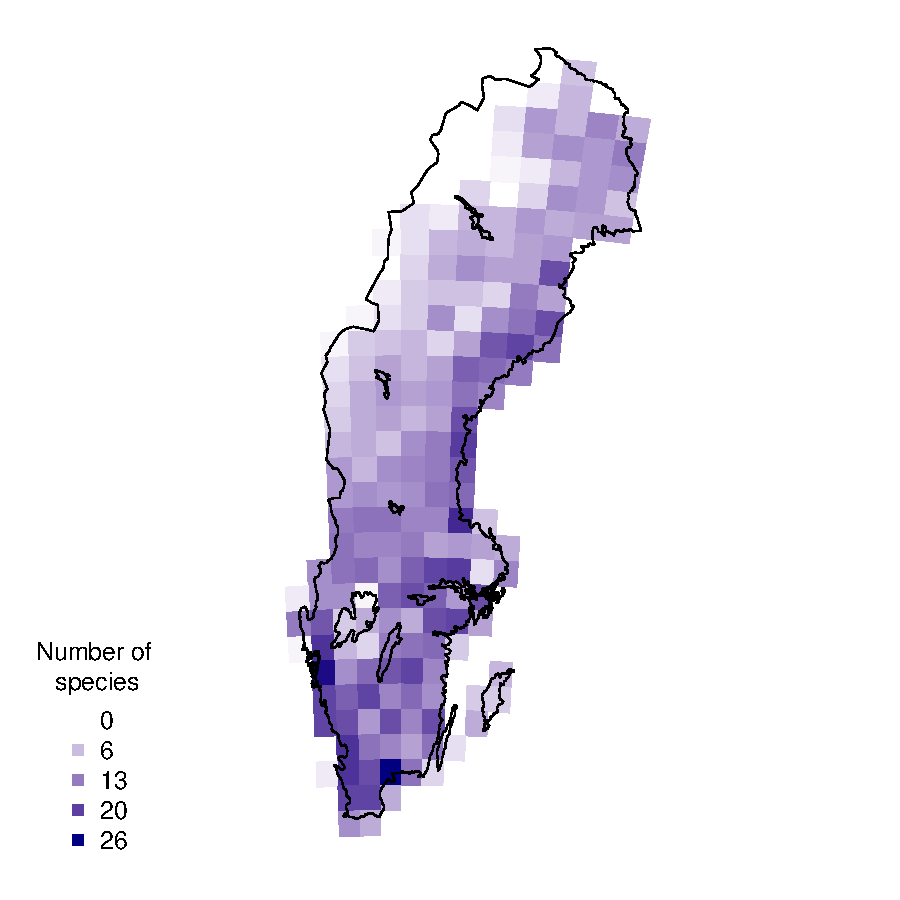
\includegraphics{r-tools-tutorial_files/figure-latex/grid-1.pdf}

\begin{Shaded}
\begin{Highlighting}[]
\FunctionTok{suppressWarnings}\NormalTok{(}\FunctionTok{par}\NormalTok{(oldpar))}
\end{Highlighting}
\end{Shaded}

We can go further by gathering the observations by latitude.

\begin{Shaded}
\begin{Highlighting}[]
\FunctionTok{library}\NormalTok{(dplyr)}
\FunctionTok{library}\NormalTok{(tidyr)}
\NormalTok{xgridded }\OtherTok{\textless{}{-}}\NormalTok{ xf}\SpecialCharTok{$}\NormalTok{data }\SpecialCharTok{\%\textgreater{}\%}
    \DocumentationTok{\#\# discard genus{-} and higher{-}level records}
    \FunctionTok{filter}\NormalTok{(rank }\SpecialCharTok{\%in\%} \FunctionTok{c}\NormalTok{(}\StringTok{"species"}\NormalTok{, }\StringTok{"subspecies"}\NormalTok{, }\StringTok{"variety"}\NormalTok{, }\StringTok{"form"}\NormalTok{, }\StringTok{"cultivar"}\NormalTok{)) }\SpecialCharTok{\%\textgreater{}\%}
    \FunctionTok{mutate}\NormalTok{(}\AttributeTok{longitude =} \FunctionTok{round}\NormalTok{(longitude }\SpecialCharTok{*} \DecValTok{4}\NormalTok{)}\SpecialCharTok{/}\DecValTok{4}\NormalTok{, }
           \AttributeTok{latitude =} \FunctionTok{round}\NormalTok{(latitude }\SpecialCharTok{*} \DecValTok{4}\NormalTok{)}\SpecialCharTok{/}\DecValTok{4}\NormalTok{) }\SpecialCharTok{\%\textgreater{}\%}
    \FunctionTok{group\_by}\NormalTok{(longitude,latitude) }\SpecialCharTok{\%\textgreater{}\%}
    \DocumentationTok{\#\# subset to vars of interest}
    \FunctionTok{select}\NormalTok{(longitude, latitude, species) }\SpecialCharTok{\%\textgreater{}\%}
    \DocumentationTok{\#\# take one row per cell per species (presence)}
    \FunctionTok{distinct}\NormalTok{() }\SpecialCharTok{\%\textgreater{}\%}
    \DocumentationTok{\#\# calculate species richness}
    \FunctionTok{mutate}\NormalTok{(}\AttributeTok{richness=}\FunctionTok{n}\NormalTok{()) }\SpecialCharTok{\%\textgreater{}\%}
    \DocumentationTok{\#\# convert to wide format (sites by species)}
    \FunctionTok{mutate}\NormalTok{(}\AttributeTok{present=}\DecValTok{1}\NormalTok{) }\SpecialCharTok{\%\textgreater{}\%}
    \FunctionTok{do}\NormalTok{(tidyr}\SpecialCharTok{::}\FunctionTok{pivot\_wider}\NormalTok{(}\AttributeTok{data=}\NormalTok{.,  }\AttributeTok{names\_from=}\NormalTok{species, }\AttributeTok{values\_from=}\NormalTok{present, }\AttributeTok{values\_fill=}\DecValTok{0}\NormalTok{)) }\SpecialCharTok{\%\textgreater{}\%}
    \FunctionTok{ungroup}\NormalTok{()}
\DocumentationTok{\#\# where a species was not present, it will have NA: convert these to 0}
\NormalTok{sppcols }\OtherTok{\textless{}{-}} \FunctionTok{setdiff}\NormalTok{(}\FunctionTok{names}\NormalTok{(xgridded),}
                   \FunctionTok{c}\NormalTok{(}\StringTok{"longitude"}\NormalTok{, }\StringTok{"latitude"}\NormalTok{, }\StringTok{"richness"}\NormalTok{))}
\NormalTok{xgridded }\OtherTok{\textless{}{-}}\NormalTok{ xgridded }\SpecialCharTok{\%\textgreater{}\%} 
  \FunctionTok{mutate\_at}\NormalTok{(sppcols, }\ControlFlowTok{function}\NormalTok{(z) }\FunctionTok{ifelse}\NormalTok{(}\FunctionTok{is.na}\NormalTok{(z), }\DecValTok{0}\NormalTok{, z))}
\end{Highlighting}
\end{Shaded}

And plot it accordingly

\begin{Shaded}
\begin{Highlighting}[]
\FunctionTok{library}\NormalTok{(ggplot2)}

\FunctionTok{ggplot}\NormalTok{(xgridded, }\FunctionTok{aes}\NormalTok{(latitude, richness)) }\SpecialCharTok{+} 
  \FunctionTok{labs}\NormalTok{(}\AttributeTok{x =} \StringTok{"Latitude (º)"}\NormalTok{, }
       \AttributeTok{y =} \StringTok{"Species richness"}\NormalTok{) }\SpecialCharTok{+}
  \FunctionTok{lims}\NormalTok{(}\AttributeTok{y =} \FunctionTok{c}\NormalTok{(}\DecValTok{0}\NormalTok{,}\DecValTok{20}\NormalTok{)) }\SpecialCharTok{+}
  \FunctionTok{geom\_point}\NormalTok{() }\SpecialCharTok{+} 
  \FunctionTok{theme\_bw}\NormalTok{()}
\end{Highlighting}
\end{Shaded}

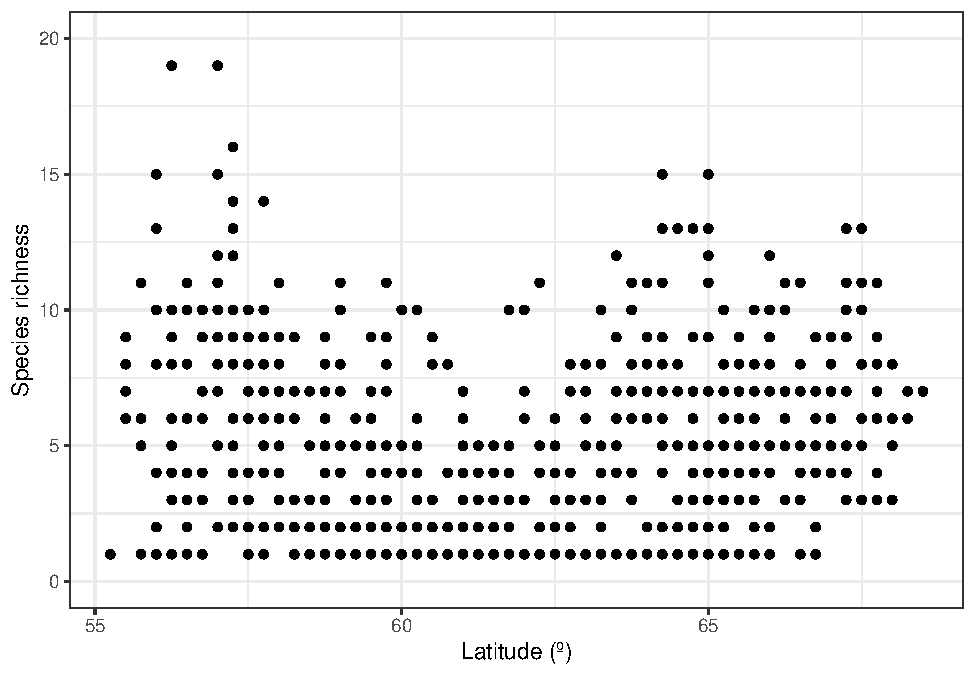
\includegraphics{r-tools-tutorial_files/figure-latex/plot_richLat-1.pdf}

\hypertarget{temporal-biodiversity-analysis}{%
\subsection{Temporal biodiversity analysis}\label{temporal-biodiversity-analysis}}

Despite the drop seen in sampling effort, we can still analyse weather there is
any trends for species over the sampled years. To do this, we first need to
check whether the spatial sampling effort was comparable across those years

\begin{Shaded}
\begin{Highlighting}[]
\NormalTok{xf}\SpecialCharTok{$}\NormalTok{data }\SpecialCharTok{\%\textgreater{}\%}
    \DocumentationTok{\#\# discard genus{-} and higher{-}level records}
    \FunctionTok{filter}\NormalTok{(rank }\SpecialCharTok{\%in\%} \FunctionTok{c}\NormalTok{(}\StringTok{"species"}\NormalTok{, }\StringTok{"subspecies"}\NormalTok{, }\StringTok{"variety"}\NormalTok{, }\StringTok{"form"}\NormalTok{, }\StringTok{"cultivar"}\NormalTok{)) }\SpecialCharTok{\%\textgreater{}\%} 
    \FunctionTok{group\_by}\NormalTok{(year) }\SpecialCharTok{\%\textgreater{}\%}
    \DocumentationTok{\#\# subset to vars of interest}
    \FunctionTok{select}\NormalTok{(year, locality) }\SpecialCharTok{\%\textgreater{}\%}
    \DocumentationTok{\#\# calculate species richness}
    \FunctionTok{mutate}\NormalTok{(}\AttributeTok{nObs =} \FunctionTok{n}\NormalTok{())}
\end{Highlighting}
\end{Shaded}

\begin{verbatim}
## # A tibble: 93,205 x 3
## # Groups:   year [5]
##     year locality                                nObs
##    <int> <chr>                                  <int>
##  1  2011 "6846840-1568800 Sjötrösk. Lillfj.utl" 16853
##  2  2009 "6340000-1286200 Göingegården"         19300
##  3  2009 ""                                     19300
##  4  2011 "6846840-1568800 Sjötrösk. Lillfj.utl" 16853
##  5  2009 "6339030-1288080 Holmagärde B st.v. 2" 19300
##  6  2009 "6339030-1288080 Holmagärde B stv. 2"  19300
##  7  2009 ""                                     19300
##  8  2010 "6321540-1301320 Ned övre kulv. Krono" 19648
##  9  2010 ""                                     19648
## 10  2009 "6466090-1409270 Nedstr Herrekvarn"    19300
## # ... with 93,195 more rows
\end{verbatim}

And we ask: can we see a trend (change = frequency of occurrence = number caught) for species X, or species Y?

\hypertarget{links-to-further-tutorials-that-could-be-of-interest}{%
\subsection{Links to further tutorials that could be of interest}\label{links-to-further-tutorials-that-could-be-of-interest}}

Link to analyses of interest -- e.g.~species distribution models, or trend analyses, or species divesity -- link to biodiversity workflow

\hypertarget{case-2}{%
\section{Case 2:}\label{case-2}}

Look at opportunistically collected citizen science data -- using the big Swedish cit science species observation data portal Artportalen.

We want to look at dragonflies -- but before we can use the observation records we need to know how the observation effort has varied over time and in space. For this we define field visits i.e.~occasions at which an observer has sampled observations -- if we have information on observer id, location id and date we can aggregate data into ``field visits''. We do this using BIRDS, and 25km grid:
Select data -- get records for Southern Sweden (Götaland) and years 2000-2010.
How has observation effort (frequency of visits) varied over time and space? -- 1) show maps as in Example 7 (all years, year 2000, 2002, 2004, 2006, 2008, 2010), 2 make also a time line plot with no. visits against years, no. of gridcells with visits against years.

We can now look at some particular species and ask whether this has changed in occurrence over time:
Plot no. records of species x and no. visits all species over years (we simply explore by comparing records for a species with no visits, can assume that species has increased of stronger positive trend than for no. visits)
Plot no. gridcells with visits for species x and no. gridcells with visits for all species over years (we simply explore by comparing records for a species with no visits, can assume that species has increased of stronger positive trend than for no. visits)
(species x: Tvåfläckad trollslända Epitheca bimaculata)

  \bibliography{references.bib}

\end{document}
